\section{System Architecture Description}
\label{sec:architecture}

The architecture of the PrimeFusion FANET framework is designed as a multi-layered system that integrates communication, blockchain, and application-level functionalities to provide a secure and efficient environment for cooperative UAV operations. A conceptual block diagram of the proposed architecture is presented in Fig. \ref{fig:architecture}.

\begin{figure}[!t]
\centering
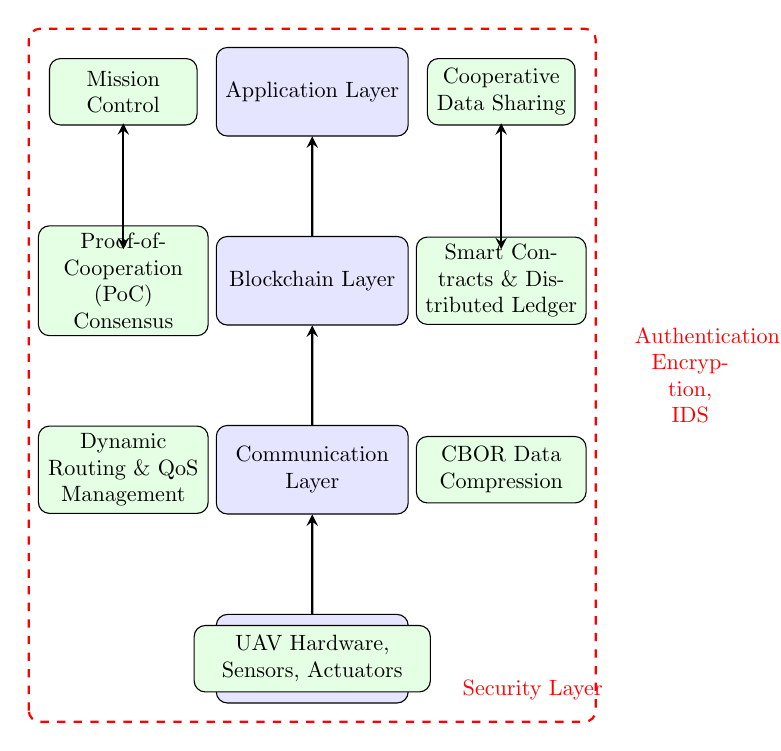
\begin{tikzpicture}[scale=0.8, transform shape]
  \tikzstyle{layer} = [rectangle, draw, fill=blue!10, text width=8em, text centered, rounded corners, minimum height=4em]
  \tikzstyle{block} = [rectangle, draw, fill=green!10, text width=7em, text centered, rounded corners, minimum height=3em]
  \tikzstyle{arrow} = [thick,->,>=stealth]

  % Layers
  \node (app) [layer] at (0,6) {Application Layer};
  \node (blockchain) [layer] at (0,3) {Blockchain Layer};
  \node (comm) [layer] at (0,0) {Communication Layer};
  \node (phy) [layer] at (0,-3) {Physical UAV Layer};

  % Blocks within layers
  \node[block, text width=6em] at (-3,6) {Mission Control};
  \node[block, text width=6em] at (3,6) {Cooperative Data Sharing};

  \node[block] at (-3,3) {Proof-of-Cooperation (PoC) Consensus};
  \node[block] at (3,3) {Smart Contracts \& Distributed Ledger};

  \node[block] at (-3,0) {Dynamic Routing \& QoS Management};
  \node[block] at (3,0) {CBOR Data Compression};
  
  \node[block, text width=10em] at (0,-3) {UAV Hardware, Sensors, Actuators};

  % Security Layer
  \draw[red, thick, dashed, rounded corners] (-4.5,-4) rectangle (4.5,7);
  \node[text=red] at (3.5,-3.5) {Security Layer};
  \node[text=red, text width=5em, align=center] at (6, 1.5) {Authentication, Encryption, IDS};

  % Arrows
  \draw[arrow] (phy) -- (comm);
  \draw[arrow] (comm) -- (blockchain);
  \draw[arrow] (blockchain) -- (app);
  \draw[arrow, <->] (-3, 3.5) -- (-3, 5.5);
  \draw[arrow, <->] (3, 3.5) -- (3, 5.5);

\end{tikzpicture}
\caption{System Architecture of the PrimeFusion FANET Framework.}
\label{fig:architecture}
\end{figure}

\subsection{Physical UAV Layer}
This foundational layer comprises the physical UAV platforms themselves, including their onboard sensors (e.g., GPS, cameras, LiDAR), actuators, flight controllers, and processing units. The capabilities of this layer directly influence the operational constraints of the network, such as flight duration, payload capacity, and available computational resources.

\subsection{Communication Layer}
The communication layer is responsible for establishing and maintaining the data links between UAVs. It is designed to be technology-agnostic, capable of operating over various wireless technologies including Wi-Fi, LoRa, and 5G/6G to suit different mission requirements (e.g., high-bandwidth vs. long-range). This layer incorporates two key components of the PrimeFusion framework:
\begin{itemize}
    \item \textbf{CBOR Data Compression:} All data destined for transmission is first processed by the CBOR encoder to minimize its size, thereby conserving bandwidth and reducing latency.
    \item \textbf{Dynamic Routing & QoS Management:} This module manages the network topology, selecting optimal routing paths based on link quality, node mobility, and Quality of Service (QoS) requirements. It ensures that high-priority data, such as flight control commands, is delivered with minimal delay.
\end{itemize}

\subsection{Blockchain Layer}
The blockchain layer serves as the decentralized trust and data integrity backbone of the framework. It consists of:
\begin{itemize}
    \item \textbf{Proof-of-Cooperation (PoC) Consensus:} The lightweight consensus mechanism that allows nodes to agree on the state of the ledger in an energy-efficient manner. It incentivizes cooperative behavior, which is essential for the stability of the FANET.
    \item \textbf{Smart Contracts & Distributed Ledger:} The immutable distributed ledger stores all critical transactions, such as authentication events, data transfers, and reputation scores. Smart contracts are used to automate and enforce operational policies and agreements between UAVs in a decentralized fashion.
\end{itemize}

\subsection{Application Layer}
This is the highest layer of the architecture, where mission-specific logic and applications reside. This includes modules for mission control, which interprets high-level objectives into actionable UAV commands, and cooperative data sharing, which enables UAVs to pool their sensor data to build a more comprehensive situational awareness. Applications at this layer interface with the blockchain layer to record and verify critical mission data.

\subsection{Security Layer}
Security is not treated as a separate layer but as a cross-cutting concern that spans the entire architecture. The security layer provides three fundamental services: decentralized, blockchain-based \textbf{authentication} to verify the identity of all participating UAVs; end-to-end \textbf{encryption} to protect the confidentiality of all communications; and a real-time \textbf{Intrusion Detection System (IDS)} that monitors network traffic for anomalous patterns and isolates malicious actors. 

